\documentclass{article}

% if you need to pass options to natbib, use, e.g.:
% \PassOptionsToPackage{numbers, compress}{natbib}
% before loading nips_2016
%
% to avoid loading the natbib package, add option nonatbib:
% \usepackage[nonatbib]{nips_2016}

%\usepackage{nips_2016}

% to compile a camera-ready version, add the [final] option, e.g.:
\usepackage[final]{nips_2016}

\usepackage[utf8]{inputenc} % allow utf-8 input
\usepackage[T1]{fontenc}    % use 8-bit T1 fonts
\usepackage{hyperref}       % hyperlinks
\usepackage{url}            % simple URL typesetting
\usepackage{booktabs}       % professional-quality tables
\usepackage{amsfonts}       % blackboard math symbols
\usepackage{amsmath}
\usepackage{nicefrac}       % compact symbols for 1/2, etc.
\usepackage{microtype}      % microtypography
\usepackage{t1enc}
\usepackage{graphicx}

\graphicspath{{./figs/}}

\title{Music generation using Deep Learning}

% The \author macro works with any number of authors. There are two
% commands used to separate the names and addresses of multiple
% authors: \And and \AND.
%
% Using \And between authors leaves it to LaTeX to determine where to
% break the lines. Using \AND forces a line break at that point. So,
% if LaTeX puts 3 of 4 authors names on the first line, and the last
% on the second line, try using \AND instead of \And before the third
% author name.

\author{
	Gábor Lant \\
	Department of Telecommunications and Media Informatics\\
	Budapest University of Technology and Economics\\
	Budapest, PA 1111 \\
	\texttt{lant.gabor98@gmail.com} \\
	\And
	Dániel M. Szalai\\
	Department of Networked Systems and Services\\
	Budapest University of Technology and Economics\\
	Budapest, PA 1111\\
	\texttt{szalaimd@gmail.com}\\
	\And
	Attila Kádár\\
	Department of Measurement and Information Systems\\
	Budapest University of Technology and Economics\\
	Budapest, PA 1111\\
	\texttt{attilaka98@gmail.com}
	%% examples of more authors
	%% \And
	%% Coauthor \\
	%% Affiliation \\
	%% Address \\
	%% \texttt{email} \\
	%% \AND
	%% Coauthor \\
	%% Affiliation \\
	%% Address \\
	%% \texttt{email} \\
	%% \And
	%% Coauthor \\
	%% Affiliation \\
	%% Address \\
	%% \texttt{email} \\
	%% \And
	%% Coauthor \\
	%% Affiliation \\
	%% Address \\
	%% \texttt{email} \\
}

\begin{document}
% \nipsfinalcopy is no longer used

\maketitle

\begin{abstract}
  In this paper we try to demonstrate how we can generate music using neural networks from sound files converted to images. The goal is to compare the performance of different types of neural networks and also different types of music to image conversions and how they affect the generated output.
\end{abstract}

\section{Problem summary}
\label{sec:summary}
Our idea was to convert our music data into pictures and then use some kind of neural network to produce similar pictures. Then we would convert our generated images back to music format and rate the quality. Originally we hoped we could use different styles of music to use as an input for our model and then it would generate a similar music but in a different style, but later we found this to be much more difficult. We will discuss this later in section~\ref{}.

\section{Data acquisition, description}
\label{sec:data}
For our data-set we had two criteria in mind: we needed .midi files and we wanted to use tracks similar to each other in style. The .midi files allow us to work with large data-sets (25- 100GB as uncompressed .wav files) without actually having to store them as .wavs thus taking up only minimal storage capacity (not counting the preprocessed files). Them being similar in style is not necessary, however we thought that it would be best for our first approach to only consider tracks from the same style. Luckily we found a well-made data-set called Magenta: Maestro~\cite{maestro}, that satisfies all our needs. Maestro is a dataset composed of over 200 hours of virtuosic piano performances.

\section{Data exploration}
\label{sec:exploration}
Our data has the following main features:
\begin{itemize}
	\item Time: Absolute time, in terms of MIDI clocks, at which this event occurs. Meta-events
	for which time is not meaningful (for example, song title, copyright information, etc.)
	have an absolute time of 0.
	\item Type/Event: Name identifying the type of the record. Record types are text consisting
	of upper and lower case letters and the underscore (``\_''), contain no embedded
	spaces, and are not enclosed in quotes.
	\item Channel: The channel identifier.
	\item Note: The currently played note (integer 21-109, a piano has 88 keys)
	\item Velocity: The matching note’s volume at the moment.
\end{itemize}
Further details at midicsv’s website~\footnote{MIDICSV: Convert MIDI File to and from CSV - Fourmilab. \url{https://www.fourmilab.ch/webtools/midicsv/}}

\section{Data preprocessing}
Here we only explain the main steps and ideas of our preprocessing, because we include a well-commented source code, that produces our actual training (70\%), validation (20\%) and test (10\%) data.

\subsection{First approach - using the midi files}
	\subsubsection{Encoding}
	We used a python package called \textbf{MidiFile} to process the midi files in the following way:
	\begin{enumerate}
		\item With the constructor of \textbf{Midifile} we can read a specific .midi file and get all the MIDI event messages presented in it. 
		\item From the aquired event messages we built a pandas dataframe which made data handling easier. The structure of the dataframe can be seen on figure \ref{fig:dframe}
		
		\begin{figure}[!htb]
			\centering
			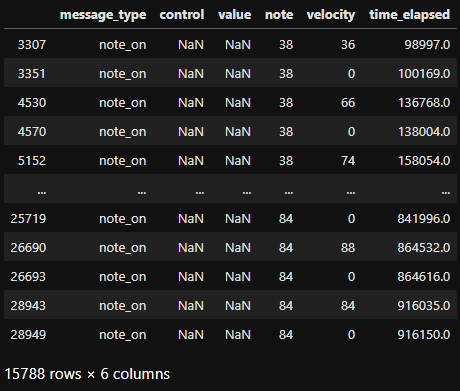
\includegraphics[width=\linewidth]{dframe.png}
			\caption{Pandas dataframe containing midi events.}
			\label{fig:dframe}
		\end{figure}
		\item The time\_elapsed column contains the same Time value as it is in the original .midi file. This column will help us to determine the starting and ending pixel of the note appearing on the generated image.
		\item We created image files, where the pitch is representsand on the y axis and the time on the x axis (we created images with size of 88x200 pixels storing approximatelly 10 seconds long pieces of music). We used three different coding methods to compare their performance: 
		\begin{itemize}
			\item In the first method we used all the 4 channels of a pixel to store different infromations about every note: its length, velocity, which instrument played that note and finally the current tempo. An example of this encoding can be seen on figure \ref{fig:encoded-1}. This encoding is very rare, since only the starting of notes are presented on these images, because the length of each note is stored in R channel. 
			\begin{figure}[!htb]
				\centering
				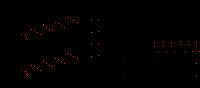
\includegraphics[width=\linewidth]{encode1.png}
				\caption{Encoding number 1.}
				\label{fig:encoded-1}
			\end{figure}
			\item The second method is very similar to the one presented above, one difference is that this encoding uses only 3 channels, because we observed that in our dataset the Tempo value is equal in every part of each song so it is not necessary to store that feature. Also in this encoding we don't store the length of notes, the value of R channel is either 125 (which means the beginning of a given note) or 255 (means that a note is sustained). So in this encoding the whole time intervall is painted where a given note is played. An example of this encoding can be seen on figure \ref{fig:encoded-2}. The index of pixels between the note shuld be painted can be determined as follows: 
				\begin{gather}
					starting\_time = tempo\times\frac{\frac{t_0}{division}}{100000} seconds \\ \nonumber
					starting\_pixel = starting\_time \times pixel\_sec \\ \nonumber
					ending\_time = tempo\times\frac{\frac{t_1}{division}}{100000} seconds \\ \nonumber
					ending\_pixel = ending\_time \times pixel\_sec, \\ \nonumber \text{where pixel\_sec is the time value corresponding to 1 pixel (it is 0.05 sec in our encoding)}
				\end{gather}
				\begin{figure}[!htb]
					\centering
					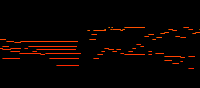
\includegraphics[width=\linewidth]{encode2.png}
					\caption{Encoding number 2.}
					\label{fig:encoded-2}
				\end{figure}
			\item The third encoding is a one-channeled version of the second one, where we doesn't store the velocity and instrument. This encoding was made only for testing the architecture with smaller dimensional inputs. This encoding is presented on figure \ref{fig:encoded-3}
				\begin{figure}[!htb]
					\centering
					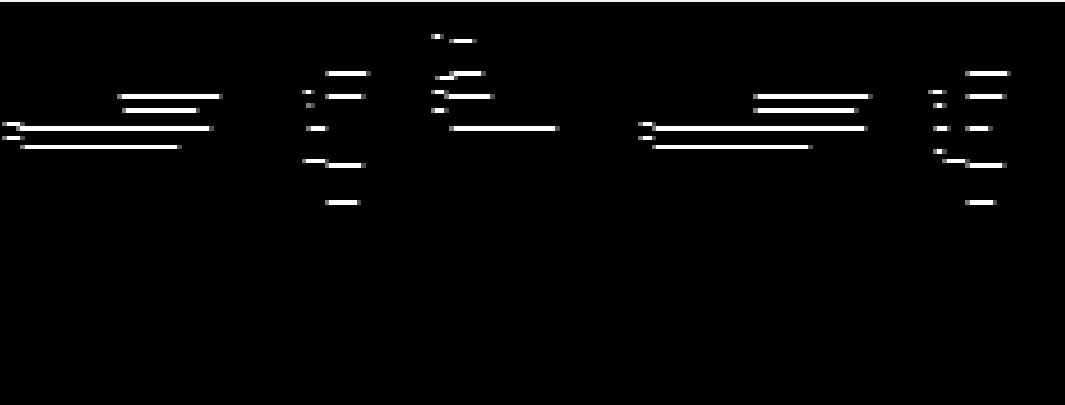
\includegraphics[width=\linewidth]{encode3.png}
					\caption{Encoding number 3.}
					\label{fig:encoded-3}
				\end{figure}
		\end{itemize}
	\end{enumerate}
	
	The code for the first encoding method can be found in \textbf{note2img.ipynb} notebook file, while the code for the second and third method can be found in \textbf{Midi2Img.ipynb} notebook file.
	\subsubsection{Decoding}
	
	After generating images with different Deep learning architectures it was necessary to create .midi files from the generated images. For this purpose we used two python packages: \textbf{Midifile} and \textbf{midiutil}. The pitch is represented on the y axis, and the duration of the note can be computed from the x axis in the following way: 
	
		\begin{gather}
		starting\_time = \frac{1000000 \times pixel\_sec \times staring\_pixel \times division}{tempo})) \\
		duration = \frac{1000000 \times length \times division}{tempo})), \\
		\text{where division is the same division which can be found in the MIDI header message} \nonumber
		\end{gather}
	
	Using the  \textbf{midifile.addNote(track, channel, note, time, duration, velocity)} function we could add notes easily to our midi files. \\ 
	
	The python code for the decoder can be found in \textbf{ImgToMidi.ipynb} notebook.
	

\subsection{Second approach - Hilbert's Curves}

In our first approach this will be the way we process the data, but we would like to note here, that we are thinking about different approaches as well. Another promising way can be the usage of Hilbert’s curves. In a nuttshell: Hilbert’s curves~\cite{hilbert} is a way to map the 1D-like spectrogram to a 2D picture, in such way, that the notes close to each other on the spectrogram will also be close on the 2D picture. This approach might work better with convolutional networks since the small matrices, parsing the picture can actually extract features that correlates more.

\subsection{Data augmentaion - MIDI approach}

As we mentioned we used midi files collected in the MAESTRO dataset, but to widen our datas at our disposal we considered using two types of data augmentation methods: 
\begin{itemize}
	\item \textbf{Transposing music: } Before generating images from audio files we used an instrument called MIDICSV~\footnote{MIDICSV: Convert MIDI File to and from CSV - Fourmilab. \url{https://www.fourmilab.ch/webtools/midicsv/}}, which beside converting midi files to csv can also transpose music (shifting the whole melody to another key). So we could produce different (shifted along $Y$ axis) images from the same MIDI file.
	
	\item \textbf{Adding noise to music: } In the real life it is also possible that a musician makes mistakes while playing ( for example playes the wrong notes ). So therefore we also added a Gaussian noise to a few notes in the music. The expected value of the noise is 0 and the standard deviation is 1 (actually the noise is a standard normal distribution). We moved the note along the y axis by the integer value of the noise added to it.
\end{itemize}

\section{folyt}

\section{Submission of papers to NIPS 2016}

\textbf{There is a new style file for papers submitted in 2016!}

NIPS requires electronic submissions.  The electronic submission site
is
\begin{center}
  \url{https://cmt.research.microsoft.com/NIPS2016/}
\end{center}

Please read carefully the instructions below and follow them
faithfully.

\subsection{Style}

Papers to be submitted to NIPS 2016 must be prepared according to the
instructions presented here. Papers may only be up to eight pages
long, including figures. Since 2009 an additional ninth page
\emph{containing only acknowledgments and/or cited references} is
allowed. Papers that exceed nine pages will not be reviewed, or in any
other way considered for presentation at the conference.

The margins in 2016 are the same as since 2007, which allow for
$\sim$$15\%$ more words in the paper compared to earlier years.

Authors are required to use the NIPS \LaTeX{} style files obtainable
at the NIPS website as indicated below. Please make sure you use the
current files and not previous versions. Tweaking the style files may
be grounds for rejection.

\subsection{Retrieval of style files}

The style files for NIPS and other conference information are
available on the World Wide Web at
\begin{center}
  \url{http://www.nips.cc/}
\end{center}
The file \verb+nips_2016.pdf+ contains these instructions and
illustrates the various formatting requirements your NIPS paper must
satisfy.

The only supported style file for NIPS 2016 is \verb+nips_2016.sty+,
rewritten for \LaTeXe{}.  \textbf{Previous style files for \LaTeX{}
  2.09, Microsoft Word, and RTF are no longer supported!}

The new \LaTeX{} style file contains two optional arguments:
\verb+final+, which creates a camera-ready copy, and \verb+nonatbib+,
which will not load the \verb+natbib+ package for you in case of
package clash.

At submission time, please omit the \verb+final+ option. This will
anonymize your submission and add line numbers to aid review.  Please
do \emph{not} refer to these line numbers in your paper as they will
be removed during generation of camera-ready copies.

The file \verb+nips_2016.tex+ may be used as a ``shell'' for writing
your paper. All you have to do is replace the author, title, abstract,
and text of the paper with your own.

The formatting instructions contained in these style files are
summarized in Sections \ref{gen_inst}, \ref{headings}, and
\ref{others} below.

\section{General formatting instructions}
\label{gen_inst}

The text must be confined within a rectangle 5.5~inches (33~picas)
wide and 9~inches (54~picas) long. The left margin is 1.5~inch
(9~picas).  Use 10~point type with a vertical spacing (leading) of
11~points.  Times New Roman is the preferred typeface throughout, and
will be selected for you by default.  Paragraphs are separated by
\nicefrac{1}{2}~line space (5.5 points), with no indentation.

The paper title should be 17~point, initial caps/lower case, bold,
centered between two horizontal rules. The top rule should be 4~points
thick and the bottom rule should be 1~point thick. Allow
\nicefrac{1}{4}~inch space above and below the title to rules. All
pages should start at 1~inch (6~picas) from the top of the page.

For the final version, authors' names are set in boldface, and each
name is centered above the corresponding address. The lead author's
name is to be listed first (left-most), and the co-authors' names (if
different address) are set to follow. If there is only one co-author,
list both author and co-author side by side.

Please pay special attention to the instructions in Section \ref{others}
regarding figures, tables, acknowledgments, and references.

\section{Headings: first level}
\label{headings}

All headings should be lower case (except for first word and proper
nouns), flush left, and bold.

First-level headings should be in 12-point type.

\subsection{Headings: second level}

Second-level headings should be in 10-point type.

\subsubsection{Headings: third level}

Third-level headings should be in 10-point type.

\paragraph{Paragraphs}

There is also a \verb+\paragraph+ command available, which sets the
heading in bold, flush left, and inline with the text, with the
heading followed by 1\,em of space.

\section{Citations, figures, tables, references}
\label{others}

These instructions apply to everyone.

\subsection{Citations within the text}

The \verb+natbib+ package will be loaded for you by default.
Citations may be author/year or numeric, as long as you maintain
internal consistency.  As to the format of the references themselves,
any style is acceptable as long as it is used consistently.

The documentation for \verb+natbib+ may be found at
\begin{center}
  \url{http://mirrors.ctan.org/macros/latex/contrib/natbib/natnotes.pdf}
\end{center}
Of note is the command \verb+\citet+, which produces citations
appropriate for use in inline text.  For example,
\begin{verbatim}
   \citet{hasselmo} investigated\dots
\end{verbatim}
produces
\begin{quote}
  Hasselmo, et al.\ (1995) investigated\dots
\end{quote}

If you wish to load the \verb+natbib+ package with options, you may
add the following before loading the \verb+nips_2016+ package:
\begin{verbatim}
   \PassOptionsToPackage{options}{natbib}
\end{verbatim}

If \verb+natbib+ clashes with another package you load, you can add
the optional argument \verb+nonatbib+ when loading the style file:
\begin{verbatim}
   \usepackage[nonatbib]{nips_2016}
\end{verbatim}

As submission is double blind, refer to your own published work in the
third person. That is, use ``In the previous work of Jones et
al.\ [4],'' not ``In our previous work [4].'' If you cite your other
papers that are not widely available (e.g., a journal paper under
review), use anonymous author names in the citation, e.g., an author
of the form ``A.\ Anonymous.''

\subsection{Footnotes}

Footnotes should be used sparingly.  If you do require a footnote,
indicate footnotes with a number\footnote{Sample of the first
  footnote.} in the text. Place the footnotes at the bottom of the
page on which they appear.  Precede the footnote with a horizontal
rule of 2~inches (12~picas).

Note that footnotes are properly typeset \emph{after} punctuation
marks.\footnote{As in this example.}

\subsection{Figures}

All artwork must be neat, clean, and legible. Lines should be dark
enough for purposes of reproduction. The figure number and caption
always appear after the figure. Place one line space before the figure
caption and one line space after the figure. The figure caption should
be lower case (except for first word and proper nouns); figures are
numbered consecutively.

You may use color figures.  However, it is best for the figure
captions and the paper body to be legible if the paper is printed in
either black/white or in color.
\begin{figure}[h]
  \centering
  \fbox{\rule[-.5cm]{0cm}{4cm} \rule[-.5cm]{4cm}{0cm}}
  \caption{Sample figure caption.}
\end{figure}

\subsection{Tables}

All tables must be centered, neat, clean and legible.  The table
number and title always appear before the table.  See
Table~\ref{sample-table}.

Place one line space before the table title, one line space after the
table title, and one line space after the table. The table title must
be lower case (except for first word and proper nouns); tables are
numbered consecutively.

Note that publication-quality tables \emph{do not contain vertical
  rules.} We strongly suggest the use of the \verb+booktabs+ package,
which allows for typesetting high-quality, professional tables:
\begin{center}
  \url{https://www.ctan.org/pkg/booktabs}
\end{center}
This package was used to typeset Table~\ref{sample-table}.

\begin{table}[t]
  \caption{Sample table title}
  \label{sample-table}
  \centering
  \begin{tabular}{lll}
    \toprule
    \multicolumn{2}{c}{Part}                   \\
    \cmidrule{1-2}
    Name     & Description     & Size ($\mu$m) \\
    \midrule
    Dendrite & Input terminal  & $\sim$100     \\
    Axon     & Output terminal & $\sim$10      \\
    Soma     & Cell body       & up to $10^6$  \\
    \bottomrule
  \end{tabular}
\end{table}

\section{Final instructions}

Do not change any aspects of the formatting parameters in the style
files.  In particular, do not modify the width or length of the
rectangle the text should fit into, and do not change font sizes
(except perhaps in the \textbf{References} section; see below). Please
note that pages should be numbered.

\section{Preparing PDF files}

Please prepare submission files with paper size ``US Letter,'' and
not, for example, ``A4.''

Fonts were the main cause of problems in the past years. Your PDF file
must only contain Type 1 or Embedded TrueType fonts. Here are a few
instructions to achieve this.

\begin{itemize}

\item You should directly generate PDF files using \verb+pdflatex+.

\item You can check which fonts a PDF files uses.  In Acrobat Reader,
  select the menu Files$>$Document Properties$>$Fonts and select Show
  All Fonts. You can also use the program \verb+pdffonts+ which comes
  with \verb+xpdf+ and is available out-of-the-box on most Linux
  machines.

\item The IEEE has recommendations for generating PDF files whose
  fonts are also acceptable for NIPS. Please see
  \url{http://www.emfield.org/icuwb2010/downloads/IEEE-PDF-SpecV32.pdf}

\item \verb+xfig+ "patterned" shapes are implemented with bitmap
  fonts.  Use "solid" shapes instead.

\item The \verb+\bbold+ package almost always uses bitmap fonts.  You
  should use the equivalent AMS Fonts:
\begin{verbatim}
   \usepackage{amsfonts}
\end{verbatim}
followed by, e.g., \verb+\mathbb{R}+, \verb+\mathbb{N}+, or
\verb+\mathbb{C}+ for $\mathbb{R}$, $\mathbb{N}$ or $\mathbb{C}$.  You
can also use the following workaround for reals, natural and complex:
\begin{verbatim}
   \newcommand{\RR}{I\!\!R} %real numbers
   \newcommand{\Nat}{I\!\!N} %natural numbers
   \newcommand{\CC}{I\!\!\!\!C} %complex numbers
\end{verbatim}
Note that \verb+amsfonts+ is automatically loaded by the
\verb+amssymb+ package.

\end{itemize}

If your file contains type 3 fonts or non embedded TrueType fonts, we
will ask you to fix it.

\subsection{Margins in \LaTeX{}}

Most of the margin problems come from figures positioned by hand using
\verb+\special+ or other commands. We suggest using the command
\verb+\includegraphics+ from the \verb+graphicx+ package. Always
specify the figure width as a multiple of the line width as in the
example below:
\begin{verbatim}
   \usepackage[pdftex]{graphicx} ...
   \includegraphics[width=0.8\linewidth]{myfile.pdf}
\end{verbatim}
See Section 4.4 in the graphics bundle documentation
(\url{http://mirrors.ctan.org/macros/latex/required/graphics/grfguide.pdf})

A number of width problems arise when \LaTeX{} cannot properly
hyphenate a line. Please give LaTeX hyphenation hints using the
\verb+\-+ command when necessary.

\subsubsection*{Acknowledgments}

Use unnumbered third level headings for the acknowledgments. All
acknowledgments go at the end of the paper. Do not include
acknowledgments in the anonymized submission, only in the final paper.

\section*{References}

References follow the acknowledgments. Use unnumbered first-level
heading for the references. Any choice of citation style is acceptable
as long as you are consistent. It is permissible to reduce the font
size to \verb+small+ (9 point) when listing the references. {\bf
  Remember that you can use a ninth page as long as it contains
  \emph{only} cited references.}
\medskip

\small


\end{document}